\documentclass{beamer}
\usepackage{textcomp}
\usepackage[utf8]{inputenc} 
\usepackage[T1]{fontenc}
\usepackage{lmodern}

%\usepackage{multimedia}
\usepackage{graphicx}
\usepackage[french]{babel}
\usetheme{PaloAlto}
\usecolortheme{crane}
\usefonttheme{structurebold}

\title[Navigation vocale]{Application des méthodes GOMS et
Keystroke à la navigation vocale}
%\logo{\includegraphics[width=1.5cm]{logo_utbm.png}}
\author[]{Paul LOCATELLI - Pierre ROGNON}
\institute[UTBM]{Université de Technologies de Belfort-Montbéliard}
\date{25 juin 2013}
%\addtobeamertemplate{footline}{~\hspace*{12cm}\insertframenumber/\inserttoœtalframenumber}


\usepackage[absolute,showboxes,overlay]{textpos}     % déclaration du package
\textblockorigin{0px}{0px}                               % origine des positions
\TPshowboxesfalse  
 % n'affiche pas le contour des textblock

\AtBeginSection[]
{
  \begin{frame}<beamer>
    \frametitle{Sommaire}
{\scriptsize\tableofcontents[currentsection]
}
  \end{frame}
}


\begin{document}

\begin{frame}{}
	
	\maketitle	
	
\end{frame}

	\section*{Introduction}

\begin{frame}{Introduction}


	\begin{columns}[c]
	
	\begin{column}{5cm}
   		\begin{itemize}
			\item Deux méthodes de navigations étudiées : clavier et souris;
			\item Troisième méthode existante: la voix;
			\item Utile pour des personnes handicapées;
			\item But: savoir si cette méthode est efficace.
		\end{itemize}
  	\end{column}
	\begin{column}{5cm}
		
\includegraphics[width=5cm]{gogol}
  	\end{column}
	
	\end{columns}
    	
\end{frame}

	\section{L'outil de reconnaissance vocale}
	
\begin{frame}{L'outil de reconnaissance vocale}

	\begin{columns}[c]
	
	\begin{column}{5cm}
   		\begin{itemize}
			\item un outil complexe et lourd;
			\item utilisation de Google Speech;
			\item facile à utiliser;
			\item indépendant de toute plateforme.
		\end{itemize}
  	\end{column}
	\begin{column}{5cm}
		
\includegraphics[width=5cm]{google-logo}
  	\end{column}
	
	\end{columns}

\end{frame}

\begin{frame}{Google Speech: fonctionnement}

	\begin{columns}[c]
	
	\begin{column}{5cm}
   		\begin{enumerate}
			\item enregistrement d'un fichier audio;
			\item envoi du fichier au serveur Google Speech;
			\item traitement du fichier par le serveur;
			\item réponse du serveur avec la phrase décodée.
		\end{enumerate}
  	\end{column}
	\begin{column}{5cm}
		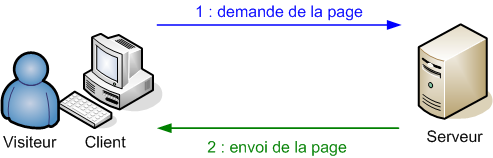
\includegraphics[width=5cm]{http}
  	\end{column}
	
	\end{columns}

\end{frame}

\begin{frame}{Enregistrement du flux: un problème}

	
	\begin{columns}[c]
	
	\begin{column}{5cm}
	\begin{itemize}
		\item l'enregistrement doit être permanent;
		\item impossible d'envoyer un flux continu au serveur;
		\item découpage en fichiers de 3 secondes après tests;
		\item utilisation de threads pour en permanence avoir des envois en cours et gagner en fluidité.
	\end{itemize}
  	\end{column}
	\begin{column}{5cm}
		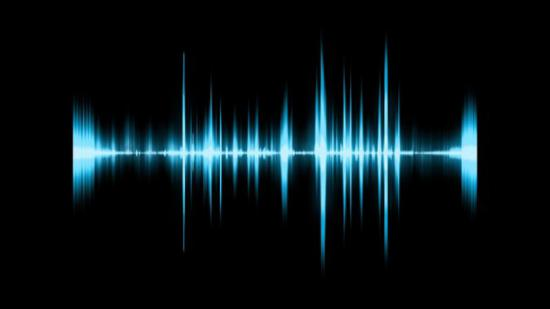
\includegraphics[width=5cm]{reconnaissance-vocale}
  	\end{column}
	
	\end{columns}

\end{frame}

	\section{L'interface logicielle}
	
\begin{frame}{L'interface logicielle}

	\begin{itemize}
		\item support nécessaire pour pouvoir mettre en place des tests de navigation vocale;
		\item choix d'une interface à la manière d'un navigateur de fichiers;
		\item éditeur de fichier texte intégré pour un autre test;
		\item choix d'une interface simple mais fonctionnelle au clavier et à la souris.
	\end{itemize}
	
\end{frame}

\begin{frame}{L'interface logicielle}

	
	\begin{columns}[c]
	
	\begin{column}{5cm}
	\begin{itemize}
		\item volonté d'utilisation possible en dehors des tests;
		\item deux modes développées, avec passage transparent de l'un à l'autre;
		\item trois parties: barre de boutons, partie principale, barre de retour de reconnaissance.
	\end{itemize}
  	\end{column}
	\begin{column}{5cm}
		\includegraphics[width=5cm]{thunar}\\
		\emph{\small Thunar, navigateur par défaut de l'environnement graphique XFCE.}
  	\end{column}
  	
  	\normalsize
	
	\end{columns}

\end{frame}

\begin{frame}{Le mode navigateur}

	\begin{columns}[c]
	
	\begin{column}{5cm}
	\begin{itemize}
		\item restriction aux simples fichiers texte et répertoires;
		\item boutons précédent, accueil, test et aide;
		\item répertoire . et .. pour répertoire courant père;
		\item aide répertoriant toutes les commandes vocales disponibles.
	\end{itemize}
  	\end{column}
	\begin{column}{5cm}
		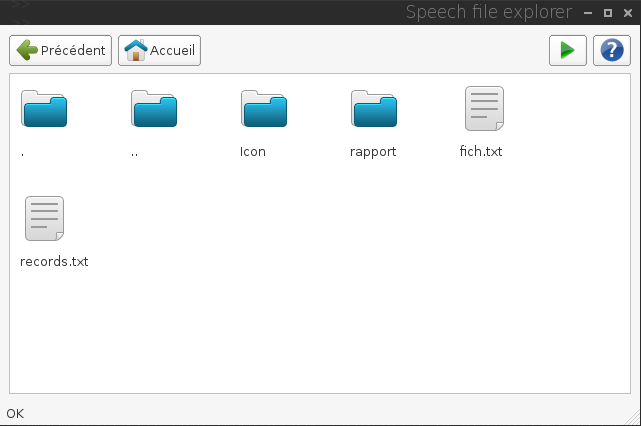
\includegraphics[width=5cm]{explorer}\\
  	\end{column}
  	
  	\normalsize
	
	\end{columns}

\end{frame}

\begin{frame}{Le mode éditeur}

	\begin{columns}[c]
	
	\begin{column}{5cm}
	\begin{itemize}
		\item bascule automatiquement lors de la sélection d'un fichier texte;
		\item même partie pour l'édition que pour la navigation;
		\item 
	\end{itemize}
  	\end{column}
	\begin{column}{5cm}
		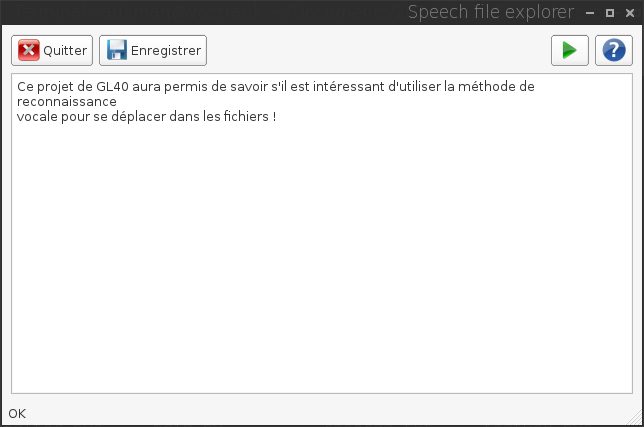
\includegraphics[width=5cm]{editor}\\
  	\end{column}
  	
  	\normalsize
	
	\end{columns}


\end{frame}




	

\end{document}


